\documentclass[a4paper,fleqn]{cas-sc}

\usepackage[utf8]{inputenc}
\usepackage[numbers]{natbib}
\usepackage{amsmath,amssymb,amsfonts}
\usepackage{booktabs}
\usepackage{graphicx}
\graphicspath{{./}{plots/}{../plots/}{./plots/}}
\usepackage{hyperref}
\usepackage{microtype}
\usepackage{lastpage}
\usepackage[section]{placeins}

\begin{document}
\let\WriteBookmarks\relax
\gdef\lastpage{\pageref{LastPage}}

% Float positioning and spacing to prevent collisions and float queuing
\setcounter{topnumber}{3}
\setcounter{bottomnumber}{2}
\setcounter{totalnumber}{5}
\renewcommand{\topfraction}{0.95}
\renewcommand{\bottomfraction}{0.85}
\renewcommand{\textfraction}{0.05}
\renewcommand{\floatpagefraction}{0.65}
\setlength{\floatsep}{20pt plus 4pt minus 2pt}
\setlength{\textfloatsep}{20pt plus 4pt minus 2pt}
\setlength{\intextsep}{16pt plus 2pt minus 2pt}

% Short title and author running heads
\shorttitle{Exact Solving Methods for Generalized Sudoku: SAT, CP, and ILP}
\shortauthors{Do Van Duc et al.}

% Title
\title[mode=title]{Solving Large-Scale Generalized Sudoku: A Comparative Study of Boolean Satisfiability, Constraint Programming, and Integer Linear Programming}

% Authors
\author{Do Van Duc}
\ead{24021410@vnu.edu.vn}

\begin{abstract}
Generalized Sudoku is a constraint satisfaction problem that can be used to study the performance of exact solving methods on problems of increasing size. Although standard $9 \times 9$ puzzles are often solved quickly by modern solvers, larger grids introduce additional computational challenges. This study compares three approaches to solving generalized Sudoku: Boolean Satisfiability (SAT), Constraint Programming (CP), and Integer Linear Programming (ILP).

For SAT, we evaluate five At-Most-One (AMO) encodings: Pairwise (Binomial), Binary, Sequential Counter, Commander, and Product. We also compare PySAT with the Glucose4 solver, Google OR-Tools CP-SAT, Gurobi Optimizer, IBM CPLEX MIP, and IBM CPLEX CP Optimizer. The benchmark suite covers grid sizes of $9 \times 9$, $16 \times 16$, $25 \times 25$, $36 \times 36$, and $49 \times 49$, with 46,530 solver runs reported across the experiments.

The results illustrate the trade-offs between encoding size and solving performance. Pairwise encoding requires no auxiliary variables but produces a quadratic number of clauses per AMO constraint. Product and Sequential Counter encodings reduce clause growth, although neither is consistently the fastest across all grid sizes. OR-Tools CP-SAT performs well on the larger instances, solving 18 of 20 tested $36 \times 36$ puzzles within the specified time limit. These findings show that solver performance depends on both the problem size and the chosen formulation. Further experiments on additional benchmark sets are needed to assess how broadly these results apply.
\end{abstract}

\begin{keywords}
Generalized Sudoku \sep Combinatorial Constraints \sep SAT Encodings \sep At-Most-One \sep Constraint Programming \sep Integer Linear Programming \sep Benchmarking
\end{keywords}

\maketitle

% =========================================================================
% 1. INTRODUCTION
% =========================================================================
\section{Introduction}
\label{sec:intro}

Constraint satisfaction problems (CSPs) are widely studied in computer science and artificial intelligence. They arise in applications such as scheduling, planning, and resource allocation. Generalized Sudoku is a useful example because its rules are simple to state, while solving larger instances can require substantial computation. For a grid of size $N \times N$, where $N = k^2$, each row, column, and $k \times k$ block must contain every symbol exactly once. The generalized problem is NP-complete when the grid size is allowed to vary, making it a useful test case for comparing exact solving methods.

This study considers three approaches to solving Sudoku:

\begin{enumerate}
    \item \textbf{Boolean Satisfiability (SAT)}: Represents the puzzle as a Boolean formula in Conjunctive Normal Form (CNF). Modern SAT solvers use Conflict-Driven Clause Learning (CDCL)~\cite{SAT_book} to guide the search and learn from conflicts.

    \item \textbf{Constraint Programming (CP)}: Represents each cell as an integer variable and expresses Sudoku rules through constraints such as \texttt{AllDifferent}.

    \item \textbf{Integer Linear Programming (ILP)}: Represents candidate cell assignments with binary variables and enforces the Sudoku rules through linear constraints.
\end{enumerate}

For SAT, an important modeling decision is how to encode cardinality constraints. In particular, an At-Most-One (AMO) constraint requires that no more than one literal in a given set is true. The Pairwise encoding expresses this requirement by adding a clause for every pair of literals. It is simple and requires no auxiliary variables, but the number of clauses grows quadratically with the size of the set. This can become expensive for larger grids.

Other encodings, including Binary, Sequential Counter, Commander, and Product~\cite{SAT_book, khanh_lecture_slides}, use different combinations of auxiliary variables and clauses. Their practical performance depends not only on the number of clauses they generate, but also on the structure of the resulting formula and how the solver processes it. Comparing these encodings can therefore help identify suitable SAT formulations for different puzzle sizes.

CP and ILP offer alternative ways to represent the same problem. CP solvers can use domain propagation and global constraints, whereas ILP solvers use linear relaxations and search procedures such as branch-and-bound and branch-and-cut. Hybrid solvers such as Google OR-Tools CP-SAT combine integer constraint modeling with SAT-based reasoning (Lazy Clause Generation~\cite{feydy2009lazy}). Their performance on generalized Sudoku may differ depending on the grid size, puzzle difficulty, and solver configuration.

This study evaluates these approaches on Sudoku grids ranging from $9 \times 9$ to $49 \times 49$. The main objectives are:

\begin{itemize}
    \item To compare five SAT AMO encodings in terms of variable counts, clause counts, encoding time, and solving time.
    \item To compare PySAT (Glucose4), OR-Tools CP-SAT, Gurobi Optimizer, IBM CPLEX MIP, and IBM CPLEX CP under the specified experimental settings.
    \item To examine how solver performance changes with grid size and identify the limitations observed in the tested instances.
\end{itemize}

The benchmark contains 46,530 reported solver runs, including 5,000 $9 \times 9$ puzzles with 17 clues and larger instances up to $49 \times 49$. The results provide an empirical comparison of the tested formulations and solvers; they are not intended to establish a universal ranking for all Sudoku instances.

The remainder of this paper is organized as follows. Section~\ref{sec:formulations} presents the mathematical formulations. Section~\ref{sec:setup} describes the experimental environment and benchmark datasets. Section~\ref{sec:results} reports the results and discusses the observed differences. Section~\ref{sec:conclusion} summarizes the findings and outlines possible future work.

% =========================================================================
% 2. PROBLEM FORMULATIONS
% =========================================================================
\section{Problem Formulations}
\label{sec:formulations}

\subsection{Generalized Sudoku Definition}
Let $k \ge 2$ be an integer and let $N = k^2$. A generalized Sudoku board has $N$ rows and $N$ columns and is divided into $N$ blocks, each containing $k \times k$ cells. The set of allowed symbols is $V = \{1,2,\ldots,N\}$. We denote a cell by $(r,c)$, where $r,c \in V$. Its block is identified by:
\begin{equation}
    B(r, c) = \left( \left\lfloor \frac{r-1}{k} \right\rfloor, \left\lfloor \frac{c-1}{k} \right\rfloor \right).
\end{equation}

An instance is specified by a set of clues
$\mathcal{C} \subseteq V \times V \times V$.
A tuple $(r,c,v) \in \mathcal{C}$ means that cell $(r,c)$ is assigned symbol $v$ in the input puzzle. A solution is a complete assignment
$\phi: V \times V \to V$ that satisfies the clues and the following rules:

\begin{enumerate}
    \item \textbf{Clues}: $\phi(r,c)=v$ for every $(r,c,v) \in \mathcal{C}$.
    \item \textbf{Rows}: Each symbol appears exactly once in every row.
    \item \textbf{Columns}: Each symbol appears exactly once in every column.
    \item \textbf{Blocks}: Each symbol appears exactly once in every $k \times k$ block.
\end{enumerate}

\subsection{Boolean Satisfiability (SAT) Encodings}
\label{sec:sat_formulation}
In the propositional formulation, each candidate assignment is represented by a Boolean variable $x_{r, c, v} \in \{0, 1\}$, which evaluates to true if and only if cell $(r, c)$ contains symbol $v$. The total number of base propositional variables is $N^3$.

Pre-assigned clues are encoded directly as unit clauses:
\begin{equation}
    x_{r, c, v} \quad \forall (r, c, v) \in \mathcal{C}.
\end{equation}
Each Sudoku constraint combines an \textit{At-Least-One} (ALO) clause and an \textit{At-Most-One} (AMO) constraint over a literal set $L = \{l_1, l_2, \dots, l_N\}$:
\begin{align}
    \text{ALO}(L) &\equiv \bigvee_{i=1}^N l_i, \label{eq:alo} \\
    \text{AMO}(L) &\equiv \sum_{i=1}^N l_i \le 1. \label{eq:amo}
\end{align}

Constraint sets~\eqref{eq:alo} and~\eqref{eq:amo} are applied to:
\begin{itemize}
    \item \textbf{Cell validity}: $L = \{x_{r, c, v} \mid v \in V\}$ for each cell $(r, c)$.
    \item \textbf{Row uniqueness}: $L = \{x_{r, c, v} \mid c \in V\}$ for each row $r$ and symbol $v$.
    \item \textbf{Column uniqueness}: $L = \{x_{r, c, v} \mid r \in V\}$ for each column $c$ and symbol $v$.
    \item \textbf{Block uniqueness}: $L = \{x_{r, c, v} \mid (r, c) \in \text{block } B\}$ for each block $B$ and symbol $v$.
\end{itemize}

While ALO yields a single disjunctive clause of length $N$, the efficiency of the SAT model depends heavily on the AMO encoding of $L$. Following the theoretical foundations and encoding classifications in~\cite{SAT_book, khanh_lecture_slides}, we evaluate five representative AMO formulations:
\begin{enumerate}
    \item \textbf{Binomial (Pairwise) Encoding}: Prohibits every pair of distinct literals:
    \begin{equation}
        \bigwedge_{1 \le i < j \le N} (\neg l_i \lor \neg l_j).
    \end{equation}
    This requires $\binom{N}{2} = \frac{N(N-1)}{2}$ binary clauses and $0$ auxiliary variables.
    
    \item \textbf{Binary Encoding}: Introduces $p = \lceil \log_2 N \rceil$ auxiliary Boolean variables $b_1, \dots, b_p$ to represent the binary index of the active literal. If $l_i$ is true, the auxiliary variables must match the binary representation of $i$, generating $N \lceil \log_2 N \rceil$ clauses and $\lceil \log_2 N \rceil$ auxiliary variables.
    
    \item \textbf{Sequential Counter Encoding}: Uses $N-1$ auxiliary variables $s_1, \dots, s_{N-1}$ to accumulate the partial sum of true literals. It generates $3N - 4$ clauses:
    \begin{equation}
        (\neg l_1 \lor s_1) \land \bigwedge_{i=2}^{N-1} \left( (\neg l_i \lor s_i) \land (\neg s_{i-1} \lor s_i) \land (\neg l_i \lor \neg s_{i-1}) \right) \land (\neg l_N \lor \neg s_{N-1}).
    \end{equation}
    
    \item \textbf{Commander Encoding}: Partitions $L$ into disjoint groups of size $g \approx 3$. A commander variable is assigned to each group to denote whether a literal in that group is satisfied, recursively enforcing AMO across groups. This yields $\mathcal{O}(N)$ clauses and $\mathcal{O}(N/g)$ auxiliary variables.
    
    \item \textbf{Product (2D Grid) Encoding}: Maps literals onto a $p \times q$ grid with $p = \lceil\sqrt{N}\rceil$ and $q = \lceil N/p \rceil$, using row and column indicators $u_1, \dots, u_p$ and $w_1, \dots, w_q$. Each literal $l_{r, c}$ implies its coordinates: $(\neg l_{r, c} \lor u_r) \land (\neg l_{r, c} \lor w_c)$, while pairwise AMO is applied along row and column projections. It requires $\mathcal{O}(N)$ clauses and $2\lceil\sqrt{N}\rceil$ auxiliary variables.
\end{enumerate}

\subsection{Constraint Programming (CP) Formulation}
In the CP formulation, the puzzle is modeled naturally with multi-valued integer variables. For each cell $(r, c)$, we define an integer variable:
\begin{equation}
    X_{r, c} \in \{1, 2, \dots, N\}.
\end{equation}
Pre-assigned clues are enforced as domain restrictions:
\begin{equation}
    X_{r, c} = v \quad \forall (r, c, v) \in \mathcal{C}.
\end{equation}
Row, column, and block uniqueness conditions are expressed directly via the global constraint \texttt{AllDifferent}:
\begin{align}
    \texttt{AllDifferent}(\{X_{r, c} \mid c \in V\}) \quad &\forall r \in V, \\
    \texttt{AllDifferent}(\{X_{r, c} \mid r \in V\}) \quad &\forall c \in V, \\
    \texttt{AllDifferent}(\{X_{r, c} \mid (r, c) \in \text{block } B\}) \quad &\forall \text{block } B.
\end{align}
This representation requires only $N^2$ integer variables and $3N$ global constraints. In this study, we evaluate Google OR-Tools CP-SAT~\cite{ortools} (using Lazy Clause Generation~\cite{feydy2009lazy}) and IBM ILOG CPLEX CP Optimizer~\cite{cplex2022}.

\subsection{Integer Linear Programming (ILP) Formulation}
In the ILP formulation, binary placement variables $y_{r, c, v} \in \{0, 1\}$ are used, where $y_{r, c, v} = 1$ indicates that cell $(r, c)$ takes value $v$. The model contains $N^3$ binary variables. Clues are fixed by setting $y_{r, c, v} = 1$ for all $(r, c, v) \in \mathcal{C}$.

The constraints are expressed as systems of linear equations:
\begin{align}
    \sum_{v=1}^N y_{r, c, v} &= 1 \quad \forall r, c \in V \quad \text{(Cell assignment)}, \label{eq:ilp_cell} \\
    \sum_{c=1}^N y_{r, c, v} &= 1 \quad \forall r, v \in V \quad \text{(Row uniqueness)}, \label{eq:ilp_row} \\
    \sum_{r=1}^N y_{r, c, v} &= 1 \quad \forall c, v \in V \quad \text{(Column uniqueness)}, \label{eq:ilp_col} \\
    \sum_{(r, c) \in \text{block } B} y_{r, c, v} &= 1 \quad \forall B, v \in V \quad \text{(Block uniqueness)}. \label{eq:ilp_blk}
\end{align}
Because Sudoku is a feasibility decision problem, the objective function is a constant dummy: $\min 0$. The model is solved using Gurobi Optimizer~\cite{gurobi2024} and IBM CPLEX MIP~\cite{cplex2022}.

% =========================================================================
% 3. EXPERIMENTAL SETUP
% =========================================================================
\section{Experimental Setup}
\label{sec:setup}

\subsection{Hardware and Software Environment}
All computational experiments were executed on my personal laptop powered by an Intel Core i5-12450H processor (8 physical cores, 12 threads, up to 4.4 GHz) with 16 GB of high-speed DDR4-3200 RAM, running 64-bit Windows 11. 

The software implementations were managed via Python 3.10+:
\begin{itemize}
    \item \textbf{PySAT (Glucose4)}: \texttt{python-sat} 1.2.9~\cite{ignatiev2018pysat}, providing bindings to Glucose 4.2.
    \item \textbf{Google OR-Tools}: Version 9.11.4210~\cite{ortools}, running CP-SAT in multi-threaded mode.
    \item \textbf{Gurobi Optimizer}: Version 11.0.3~\cite{gurobi2024}, academic license, solved with default presolve and dual simplex/branch-and-cut.
    \item \textbf{IBM ILOG CPLEX}: Optimization Studio 22.1.1~\cite{cplex2022} (via \texttt{docplex} and \texttt{cplex}), evaluated under both MIP and CP Optimizer engines.
\end{itemize}

\subsection{Benchmark Datasets}
To evaluate performance and scalability as grid sizes grow, we tested five puzzle dimensions:
\begin{enumerate}
    \item \textbf{$9 \times 9$ Puzzles}: 5,000 minimal 17-clue puzzles from Gordon Royle's dataset of 9x9 Sudoku instances~\cite{royle2014minimum}.
    \item \textbf{$16 \times 16$ Puzzles}: 100 randomly generated puzzles with guaranteed unique solutions ($k = 4$).
    \item \textbf{$25 \times 25$ Puzzles}: 40 hard puzzles ($k = 5$).
    \item \textbf{$36 \times 36$ Puzzles}: 20 large-scale puzzles ($k = 6$).
    \item \textbf{$49 \times 49$ Puzzles}: 10 very large puzzles ($k = 7$).
\end{enumerate}
In total, the benchmark comprises 46,530 solver runs.

\subsection{Evaluation Protocol and Tiered Timeouts}
Because solving time increases rapidly with grid size $N$, we set tiered timeout limits to prevent excessive waiting times while ensuring a fair comparison:
\begin{itemize}
    \item $9 \times 9$: 3.0 s per puzzle
    \item $16 \times 16$: 8.0 s per puzzle
    \item $25 \times 25$: 20.0 s per puzzle
    \item $36 \times 36$: 35.0 s per puzzle
    \item $49 \times 49$: 50.0 s per puzzle
\end{itemize}
Every solver invocation records wall-clock time, encoding time, model variable count, constraint count, and outcome status (\texttt{OPTIMAL}, \texttt{FEASIBLE}, or \texttt{TIMEOUT}). All verified solutions were validated by an independent checker.

% =========================================================================
% 4. COMPUTATIONAL RESULTS AND DISCUSSION
% =========================================================================
\section{Computational Results and Discussion}
\label{sec:results}

\subsection{Ablation Study: SAT AMO Encodings}
Table~\ref{tab:sat_runtime_comparison} reports the average solving runtime (in seconds) for each of the five SAT AMO encodings across all grid sizes using the Glucose4 engine. Table~\ref{tab:sat_ablation} provides a detailed ablation breakdown showing average variable counts, clause counts, encoding time, and solving time.

% --- TABLE 1: SAT RUNTIME COMPARISON ---
\begin{table}[t]
\centering
\caption{The runtime of different SAT encoding methods (seconds) on PySAT Glucose4.}
\label{tab:sat_runtime_comparison}
\begin{tabular}{lrrrrr}
\toprule
\textbf{Grid ($N \times N$)} & \textbf{Binomial} & \textbf{Binary} & \textbf{Sequential Counter} & \textbf{Commander} & \textbf{Product} \\
\midrule
9x9 (5,000 instances)   & 0.0127 & 0.0125 & 0.0077 & \textbf{0.0069} & 0.0083 \\
16x16 (100 instances)   & 0.0954 & 0.0599 & 0.0458 & 0.0507 & \textbf{0.0448} \\
25x25 (40 instances)    & 0.6248 & 0.3052 & 0.2318 & 0.2556 & \textbf{0.2113} \\
36x36 (20 instances)    & 4.2537 & 2.4044 & \textbf{0.5310} & 0.7863 & 1.8947 \\
49x49 (10 instances)    & 8.6557 & 2.1301 & 1.3632 & 2.4676 & \textbf{1.3259} \\
\bottomrule
\end{tabular}
\end{table}

% --- TABLE 2: SAT ABLATION STUDY ---
\begin{table}[t]
\centering
\small
\caption{Ablation study of five SAT AMO encodings across Sudoku grid sizes.}
\label{tab:sat_ablation}
\resizebox{\textwidth}{!}{%
\begin{tabular}{llrrrrr}
\toprule
\textbf{Size ($N$)} & \textbf{AMO Method} & \textbf{Avg Vars} & \textbf{Avg Clauses} & \textbf{Encode Time (ms)} & \textbf{Solve Time (ms)} & \textbf{Total Time (ms)} \\
\midrule
9 & Binary             & 2,025   & 12,005       & 6.75  & 5.79   & 12.54 \\
9 & Commander          & 1,701   & 8,117        & 2.53  & 4.35   & 6.87 \\
9 & Pairwise (Binom.)  & 729     & 12,005       & 7.68  & 4.97   & 12.65 \\
9 & Product            & 2,673   & 8,117        & 3.96  & 4.37   & 8.34 \\
9 & Sequential         & 3,321   & 7,793        & 3.40  & 4.28   & 7.68 \\
\midrule
16 & Binary            & 8,192   & 66,666       & 32.52 & 27.33  & 59.85 \\
16 & Commander         & 10,240  & 54,378       & 26.81 & 23.92  & 50.73 \\
16 & Pairwise (Binom.) & 4,096   & 124,010      & 58.18 & 37.18  & 95.36 \\
16 & Product           & 12,288  & 46,186       & 24.91 & 19.87  & 44.77 \\
16 & Sequential        & 19,456  & 46,186       & 24.72 & 21.08  & 45.81 \\
\midrule
25 & Binary            & 28,125  & 315,313      & 170.56 & 134.67 & 305.23 \\
25 & Commander         & 38,125  & 237,813      & 125.48 & 130.11 & 255.59 \\
25 & Pairwise (Binom.) & 15,625  & 752,813      & 400.44 & 224.40 & 624.84 \\
25 & Product           & 40,625  & 177,813      & 86.61  & 124.70 & 211.31 \\
25 & Sequential        & 75,625  & 180,313      & 86.54  & 145.23 & 231.77 \\
\midrule
36 & Binary            & 77,760  & 1,125,722    & 519.37 & 8,578.80 & 8,923.53 \\
36 & Commander         & 108,864 & 783,578      & 482.54 & 9,063.16 & 9,339.74 \\
36 & Pairwise (Binom.) & 46,656  & 3,271,898    & 1,919.61 & 7,373.93 & 8,865.60 \\
36 & Product           & 108,864 & 534,746      & 295.65 & 8,327.35 & 8,515.77 \\
36 & Sequential        & 228,096 & 545,114      & 284.36 & 9,012.30 & 9,148.29 \\
\midrule
49 & Binary            & 175,273 & 2,834,823    & 1,105.99 & 10,976.85 & 11,704.12 \\
49 & Commander         & 280,917 & 2,412,247    & 1,520.91 & 10,936.09 & 11,974.11 \\
49 & Pairwise (Binom.) & 117,649 & 11,305,551   & 5,538.64 & 13,152.95 & 16,924.60 \\
49 & Product           & 252,105 & 1,355,807    & 819.48   & 10,531.44 & 11,060.76 \\
49 & Sequential        & 578,641 & 1,384,619    & 779.45   & 10,585.12 & 11,090.55 \\
\bottomrule
\end{tabular}%
}
\end{table}

As shown in Table~\ref{tab:sat_runtime_comparison} and Table~\ref{tab:sat_ablation}, the choice of At-Most-One (AMO) encoding greatly affects both the formula size and the solving efficiency. We present two evaluation perspectives: Table~\ref{tab:sat_runtime_comparison} shows the raw solving runtime on completed instances, while Table~\ref{tab:sat_ablation} and Figure~\ref{fig:runtime_sat} show the Penalized Average Runtime (PAR-1), which includes timeout penalties alongside formula metrics.

The results highlight several key trade-offs:

\paragraph{Clause Growth and Linear-Clause Encodings}
The Binomial (Pairwise) encoding does not add auxiliary variables, keeping the base variable count at $N^3$ (e.g., 729 variables at $9 \times 9$ and 117,649 variables at $49 \times 49$). However, this leads to a rapid quadratic increase in clauses: the number of clauses escalates from 12,005 at $9 \times 9$ to more than 11.3 million clauses at $49 \times 49$ (Figure~\ref{fig:clauses_comparison}). Consequently, generating the CNF formula alone takes 5.54 seconds on $49 \times 49$, and checking this vast number of clauses slows down the SAT solver significantly, resulting in an average PAR-1 runtime of 16.92 seconds (Table~\ref{tab:sat_ablation}). In contrast, both Product and Sequential Counter encodings keep clause growth linear ($\mathcal{O}(N)$ per constraint set). At $49 \times 49$, Product generates only 1,355,807 clauses---representing \textbf{88.0\% fewer clauses} than Binomial. Sequential Counter produces a similar clause count (1,384,619 clauses).

\begin{figure}[!t]
    \centering
    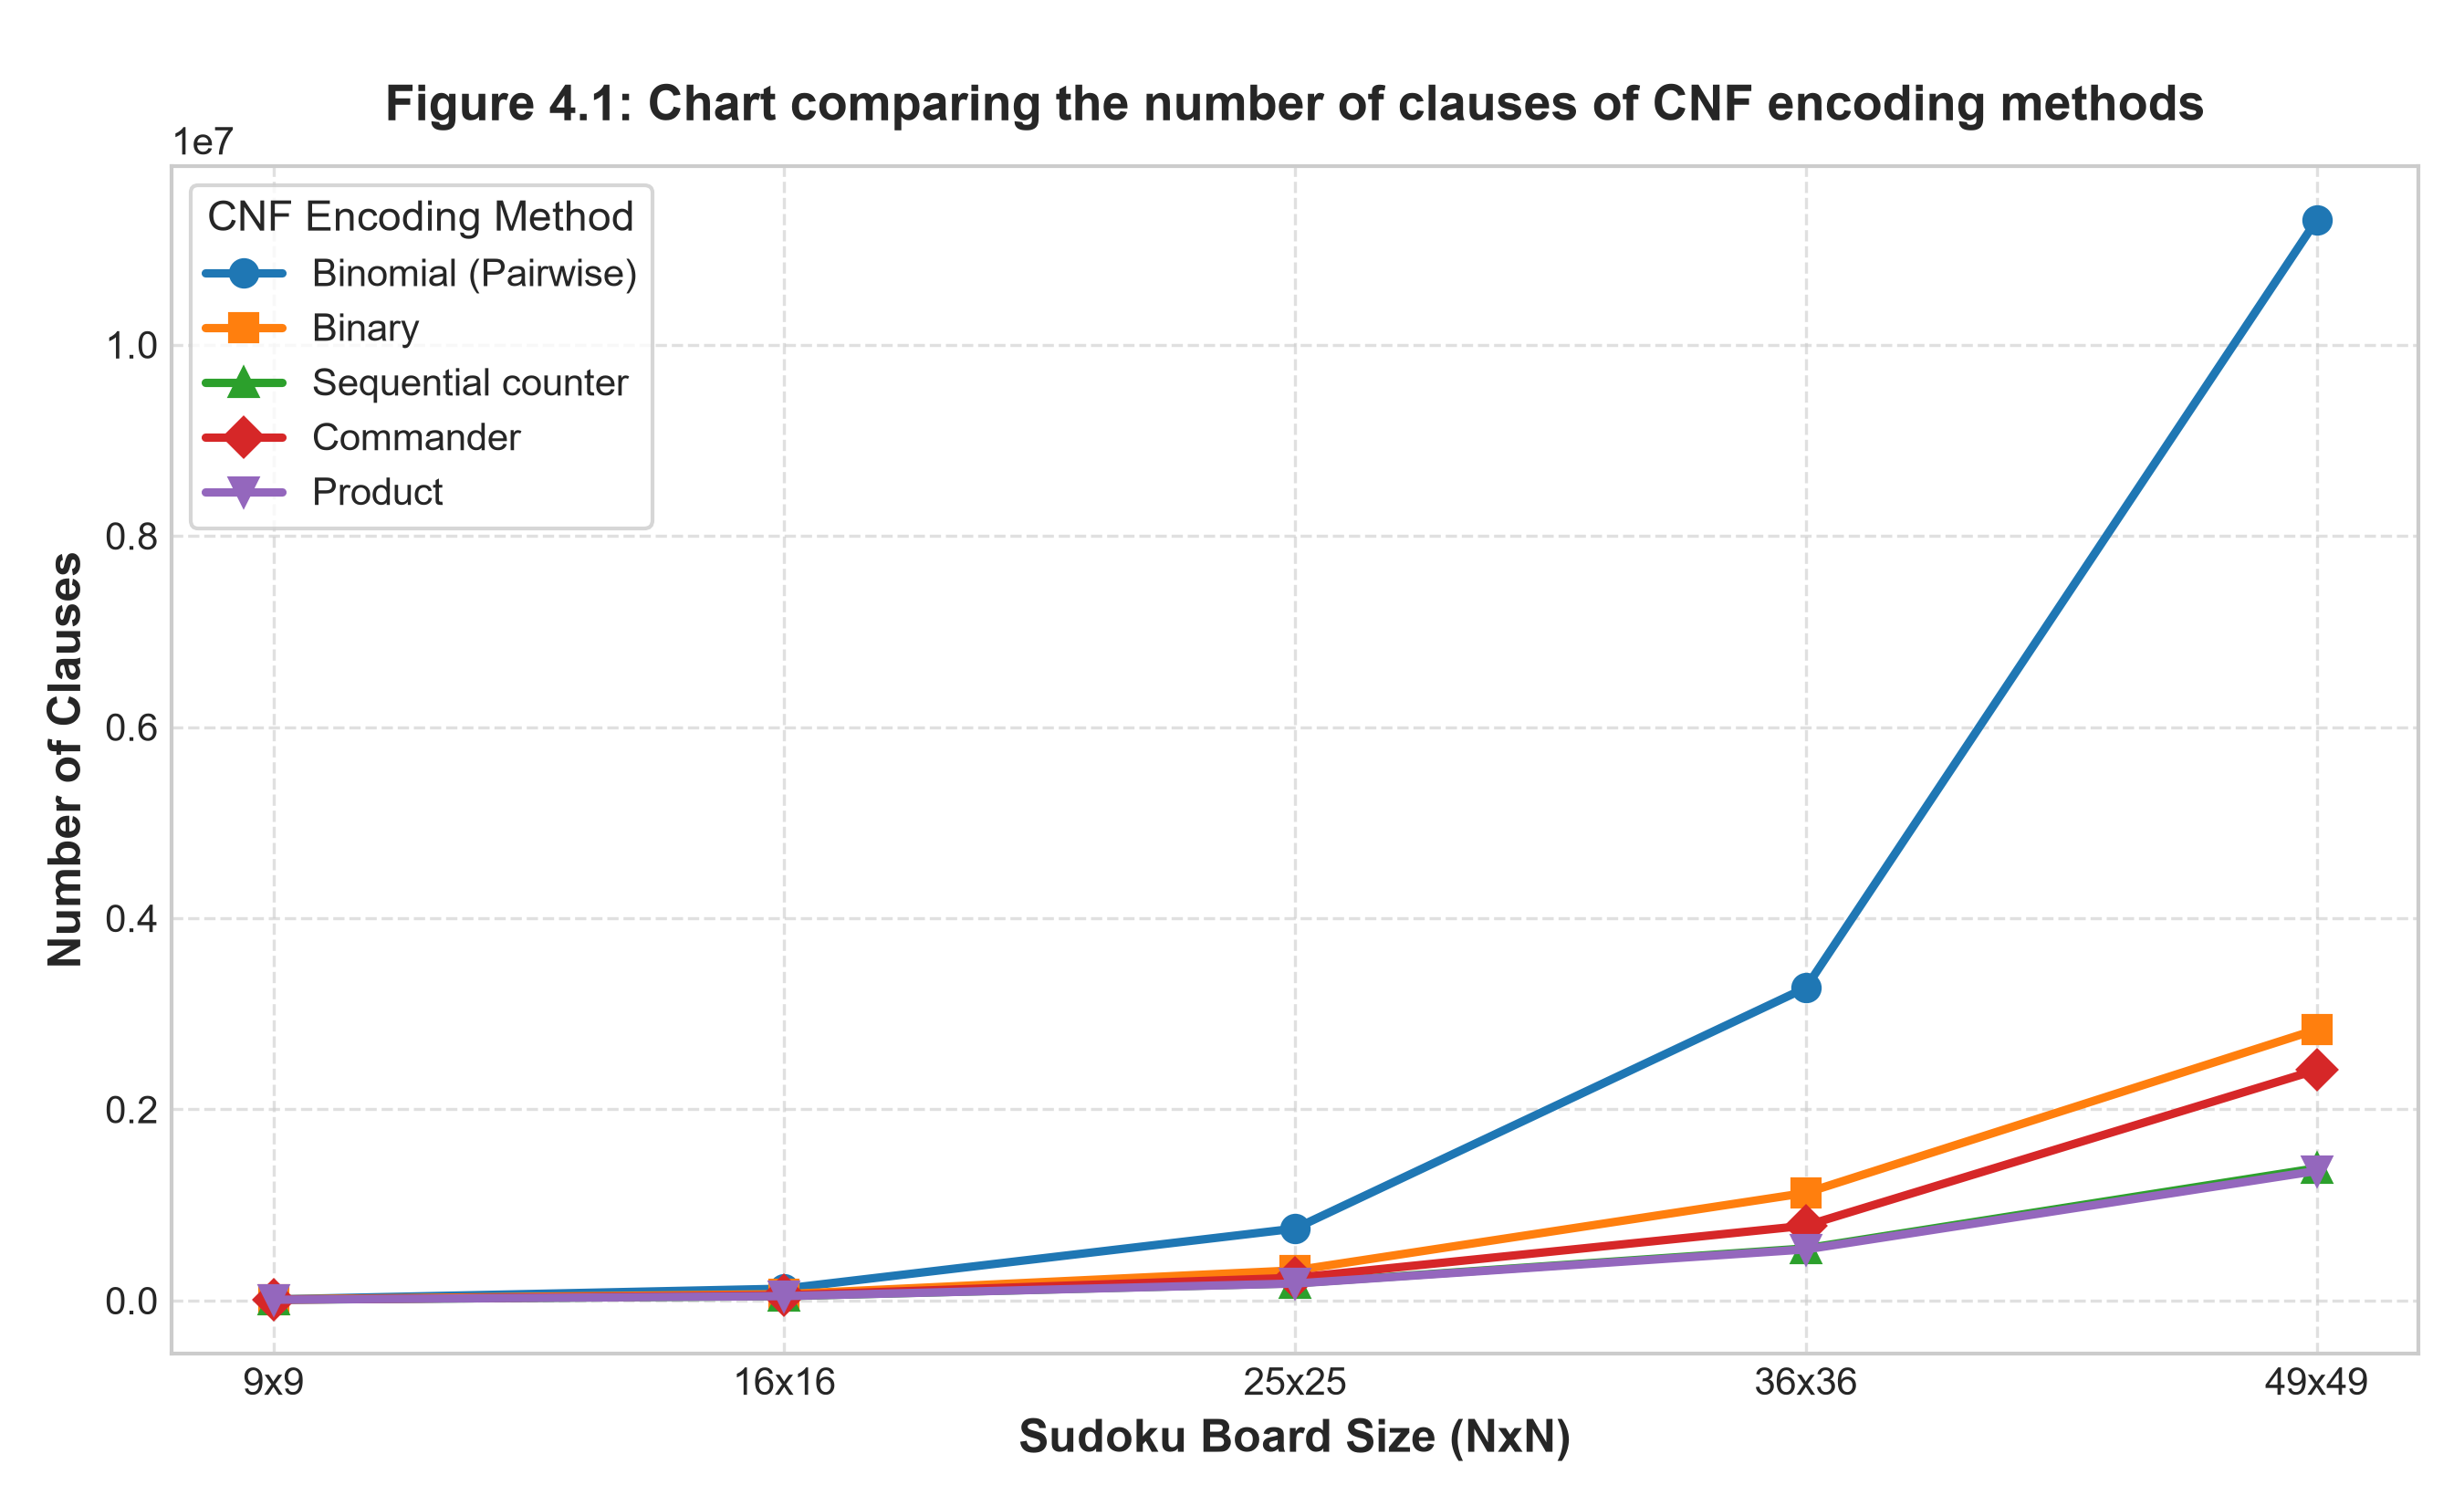
\includegraphics[width=0.58\textwidth]{fig_4_1_clauses_comparison.png}
    \vspace{2mm}
    \caption{Comparison of clause counts generated by the five SAT AMO encodings across grid sizes.}
    \label{fig:clauses_comparison}
\end{figure}

\paragraph{Auxiliary Variable Trade-off}
While Sequential Counter achieves linear clause growth, it requires a chain of $N-1$ helper variables per constraint, resulting in 578,641 total variables at $49 \times 49$ (Figure~\ref{fig:variables_comparison}). Product encoding balances this trade-off effectively: by organizing candidate literals into a 2D grid ($\lceil\sqrt{N}\rceil \times \lceil N/\lceil\sqrt{N}\rceil\rceil$), it introduces only $2\lceil\sqrt{N}\rceil$ helper variables per constraint (252,105 total variables at $49 \times 49$).

\begin{figure}[!t]
    \centering
    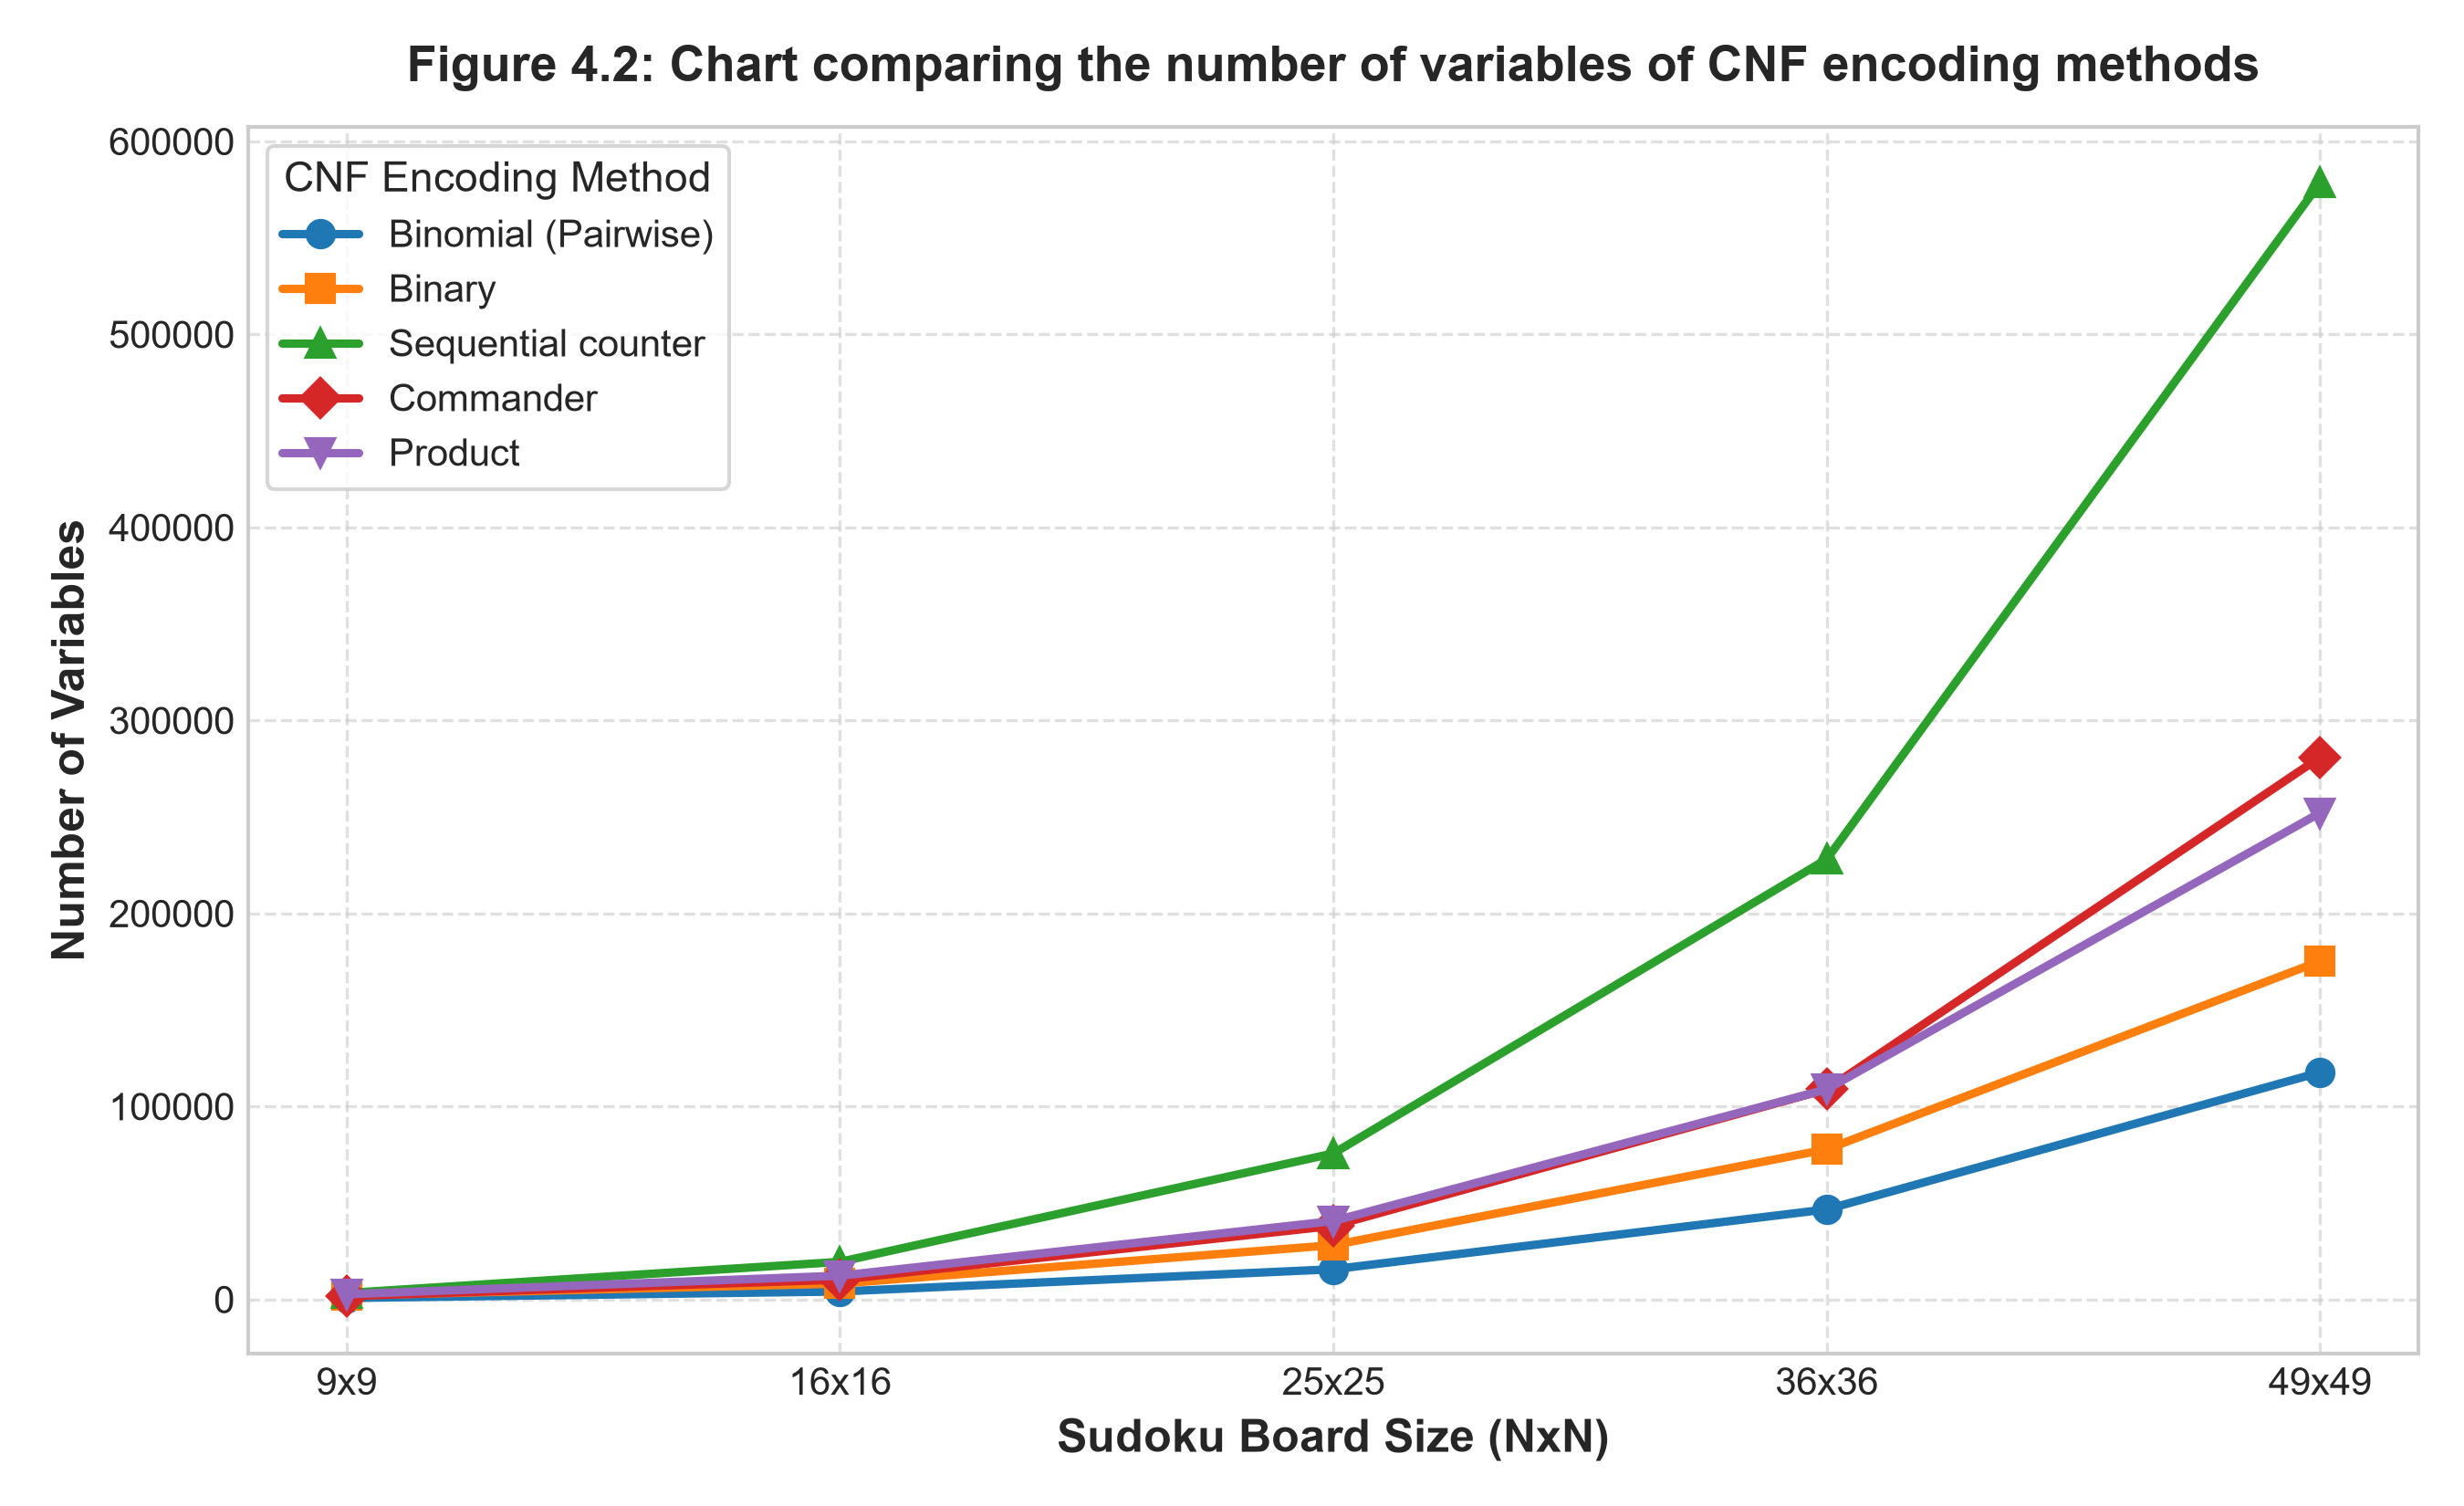
\includegraphics[width=0.58\textwidth]{fig_4_2_variables_comparison.png}
    \vspace{2mm}
    \caption{Comparison of base and auxiliary variable counts across SAT AMO encodings.}
    \label{fig:variables_comparison}
\end{figure}

\paragraph{Solving Speed}
As shown in Figure~\ref{fig:runtime_sat}, Product encoding achieved the lowest overall runtime on almost all medium and large grids (2.13 times faster than Binomial on $16 \times 16$, 2.96 times faster on $25 \times 25$, and the lowest PAR-1 solving time of 11.06 seconds on $49 \times 49$). Sequential Counter also performed well, solving finished $36 \times 36$ puzzles in an average of 0.531 seconds (Table~\ref{tab:sat_runtime_comparison}).

\begin{figure}[!t]
    \centering
    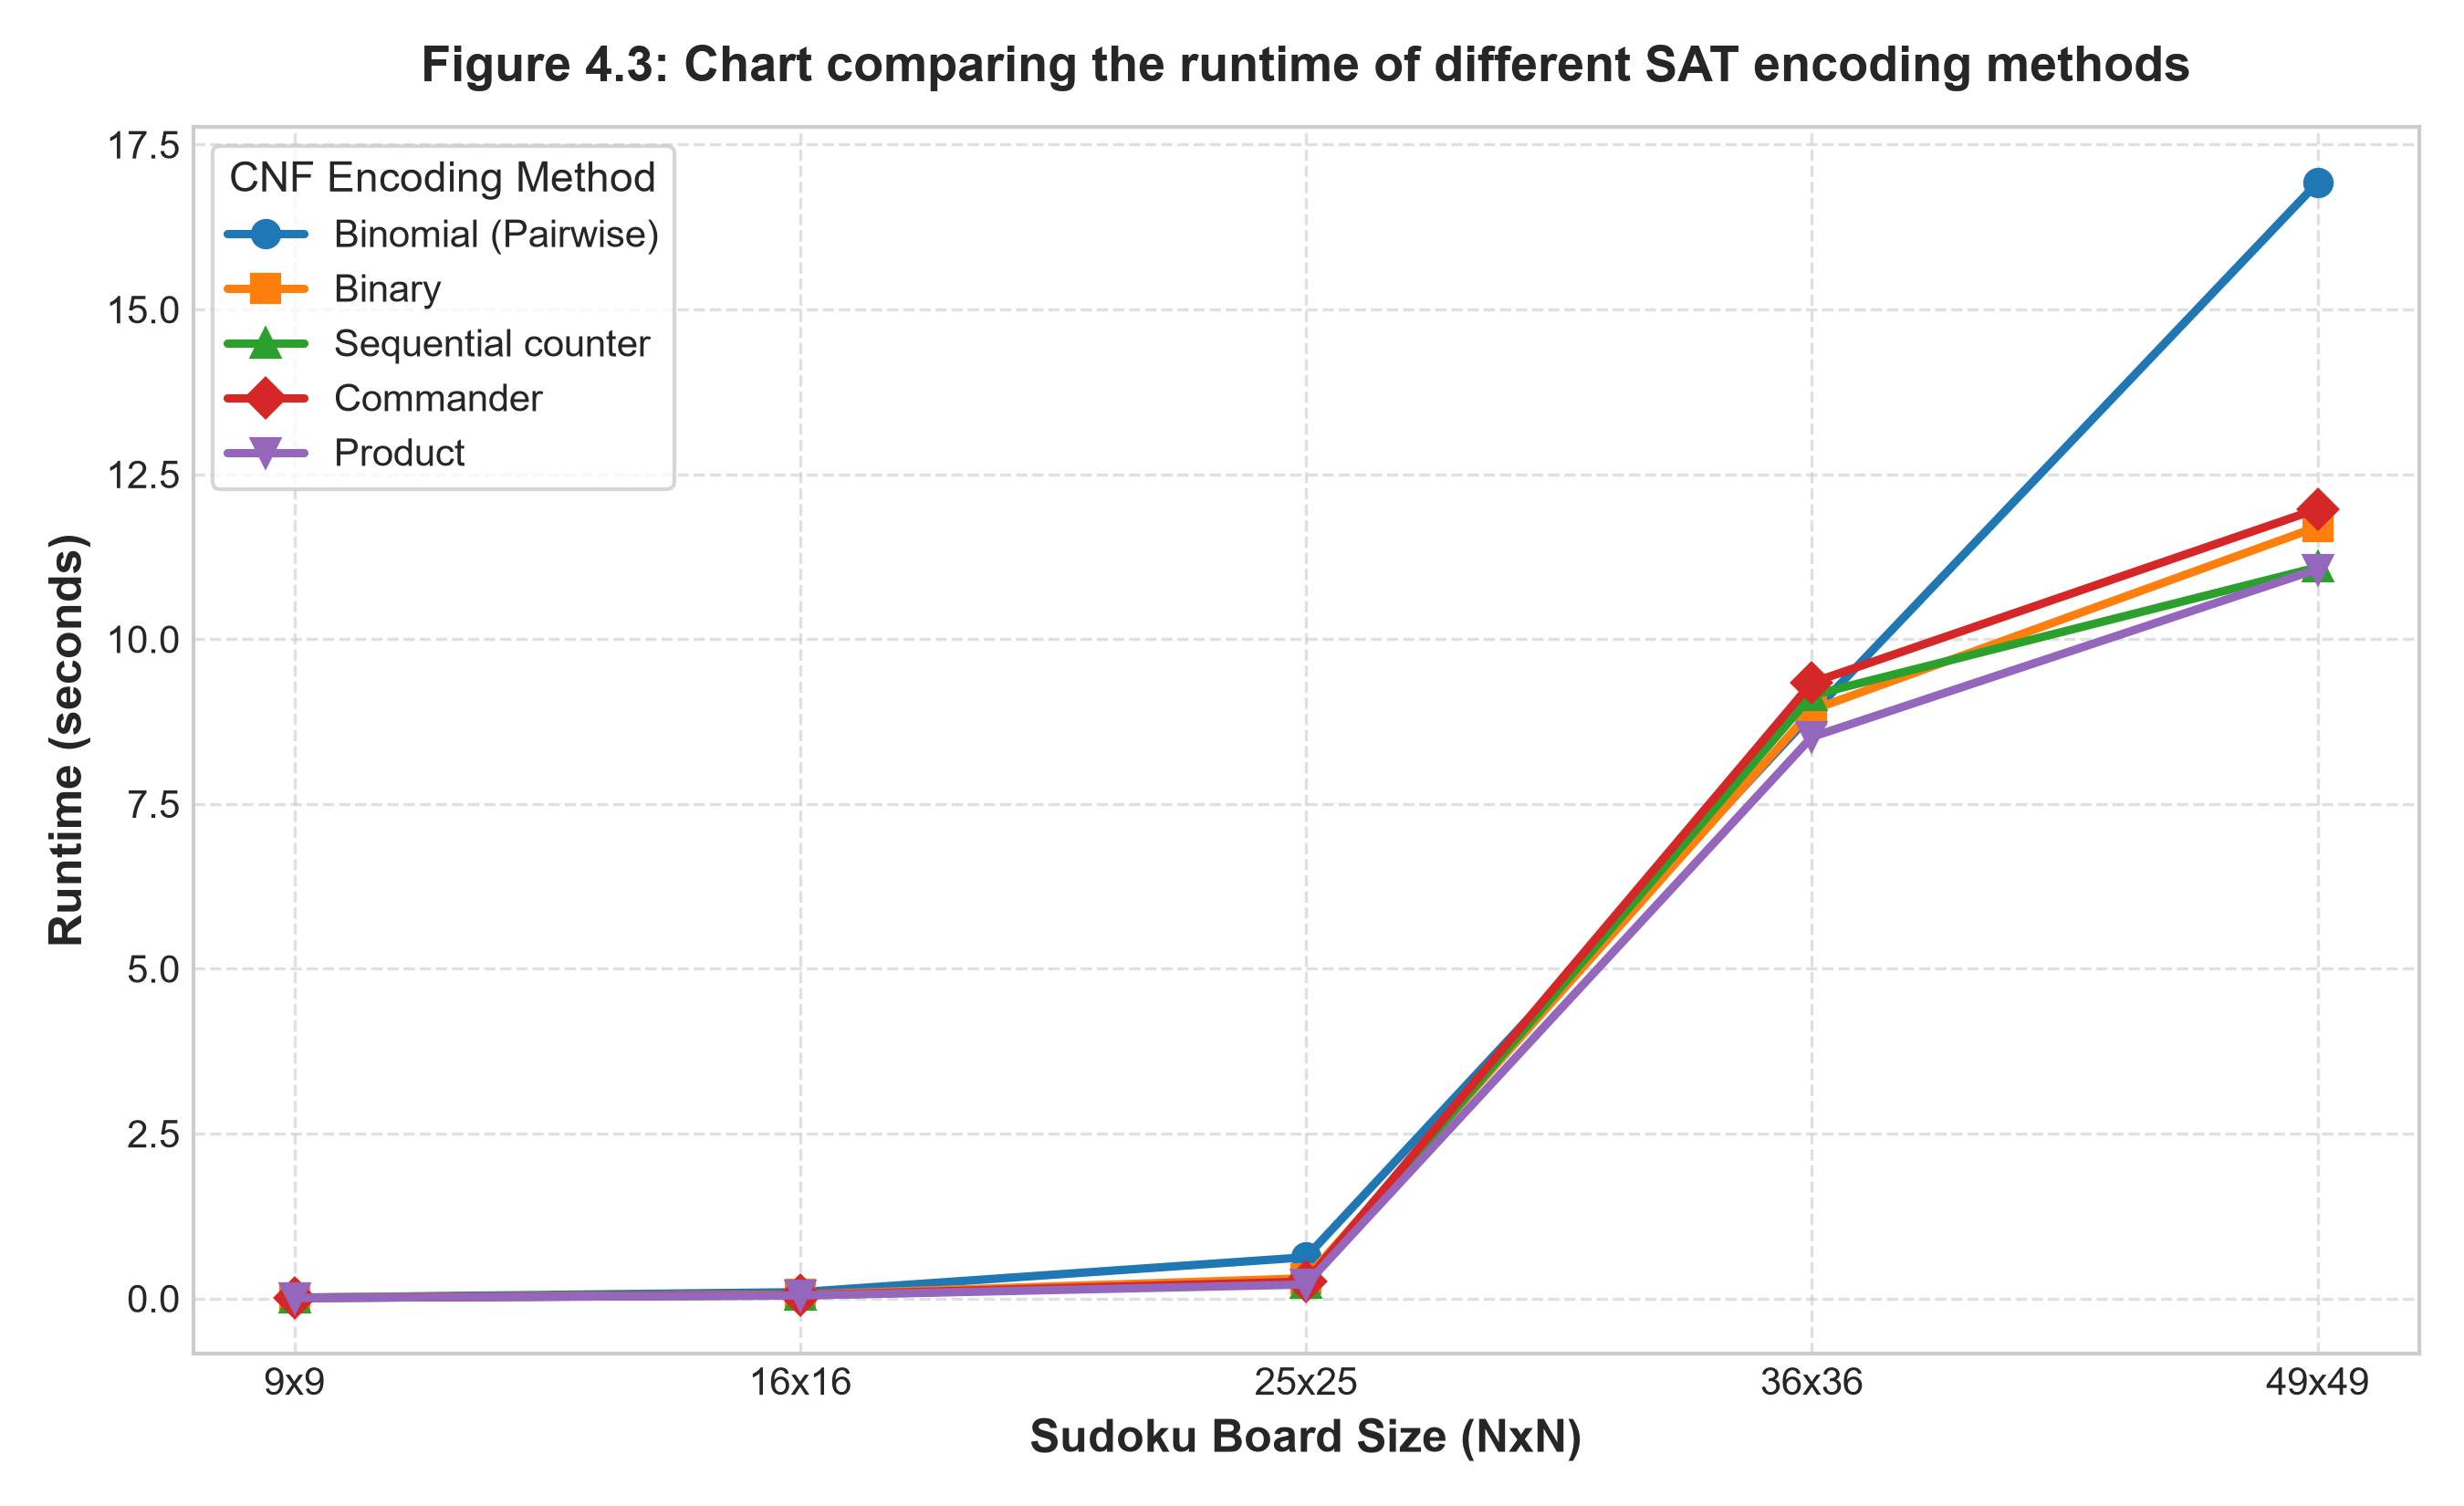
\includegraphics[width=0.58\textwidth]{fig_4_3_runtime_sat.png}
    \vspace{2mm}
    \caption{Penalized Average Runtime (PAR-1 in seconds) of the five SAT AMO encodings as grid size increases from $9 \times 9$ to $49 \times 49$ on PySAT Glucose4.}
    \label{fig:runtime_sat}
\end{figure}

\clearpage
\subsection{Cross-Paradigm Comparison: SAT vs. CP vs. ILP}
Table~\ref{tab:cross_solvers} and Figure~\ref{fig:runtime_solvers} compare the three solving paradigms: SAT (PySAT Glucose4 with Sequential Counter), Constraint Programming (Google OR-Tools CP-SAT and IBM CPLEX CP), and Integer Linear Programming (Gurobi Optimizer and IBM CPLEX MIP), running under identical hardware and tiered timeout limits.

The results show clear differences in performance across grid sizes:
\begin{itemize}
    \item \textbf{Small Grids ($9 \times 9$ and $16 \times 16$)}: All five solvers solved 100.0\% of the puzzles across the 5,000 minimal 17-clue $9 \times 9$ instances and 100 $16 \times 16$ instances. Google OR-Tools CP-SAT delivered the fastest solving times (4.25 ms on $9 \times 9$ and 39.19 ms on $16 \times 16$). Commercial ILP (Gurobi at 6.31 ms and 46.02 ms) and pure SAT (Glucose4 at 7.68 ms and 45.81 ms) followed closely, while CPLEX MIP and CPLEX CP were slightly slower due to startup overhead.
    
    \item \textbf{Medium Grids ($25 \times 25$)}: At this size, the solvers began to show major differences. Google OR-Tools CP-SAT remained the fastest, solving all 40 instances in an average of 97.51 ms. SAT with Sequential Counter ranked second at 231.77 ms, running over 7 to 11 times faster than the commercial ILP solvers (CPLEX MIP at 1,674.56 ms and Gurobi Optimizer at 2,684.57 ms). CPLEX CP started to struggle, timing out on 4 instances (90.0\% success rate, 2,951.36 ms).
    
    \item \textbf{Large-Scale Grids ($36 \times 36$ and $49 \times 49$)}: At $36 \times 36$, the puzzles became much harder to solve. Google OR-Tools CP-SAT showed high reliability, solving \textbf{18 of 20 instances (90.0\%)} with an average runtime of 5,321.63 ms. In comparison, Gurobi, CPLEX MIP, and Glucose4 each solved 15 of 20 instances (75.0\%, runtimes $\approx 9.1 - 9.3$ s), while CPLEX CP solved only 13 of 20 instances (65.0\%, 12,690.12 ms). At $49 \times 49$, all solvers converged to an 80.0\% completion rate, with OR-Tools CP-SAT maintaining the lowest PAR-1 runtime (10,035.57 ms).
\end{itemize}

% --- TABLE 3: CROSS SOLVER COMPARISON ---
\begin{table}[t]
\centering
\small
\caption{Cross-paradigm comparison of SAT, CP, and ILP solvers on generalized Sudoku (PAR-1 metric).}
\label{tab:cross_solvers}
\resizebox{\textwidth}{!}{%
\begin{tabular}{llrrrrr}
\toprule
\textbf{Grid ($N$)} & \textbf{Solver / Paradigm} & \textbf{Solved} & \textbf{Success Rate} & \textbf{Variables} & \textbf{Constraints} & \textbf{Total Time (ms)} \\
\midrule
9  & OR-Tools CP-SAT (CP)    & 5,000/5,000 & \textbf{100.0\%} & 81      & 44        & \textbf{4.25} \\
9  & Gurobi Optimizer (ILP)  & 5,000/5,000 & 100.0\%          & 729     & 341       & 6.31 \\
9  & Glucose4 (SAT - Seq)    & 5,000/5,000 & 100.0\%          & 3,321   & 7,793     & 7.68 \\
9  & CPLEX MIP (ILP)         & 5,000/5,000 & 100.0\%          & 729     & 341       & 21.38 \\
9  & CPLEX CP (CP)           & 5,000/5,000 & 100.0\%          & 81      & 44        & 43.65 \\
\midrule
16 & OR-Tools CP-SAT (CP)    & 100/100     & \textbf{100.0\%} & 256     & 154       & \textbf{39.19} \\
16 & CPLEX CP (CP)           & 100/100     & 100.0\%          & 256     & 154       & 40.27 \\
16 & Glucose4 (SAT - Seq)    & 100/100     & 100.0\%          & 19,456  & 46,186    & 45.81 \\
16 & Gurobi Optimizer (ILP)  & 100/100     & 100.0\%          & 4,096   & 1,130     & 46.02 \\
16 & CPLEX MIP (ILP)         & 100/100     & 100.0\%          & 4,096   & 1,130     & 82.80 \\
\midrule
25 & OR-Tools CP-SAT (CP)    & 40/40       & \textbf{100.0\%} & 625     & 388       & \textbf{97.51} \\
25 & Glucose4 (SAT - Seq)    & 40/40       & 100.0\%          & 75,625  & 180,312   & 231.77 \\
25 & CPLEX MIP (ILP)         & 40/40       & 100.0\%          & 15,625  & 2,813     & 1,674.56 \\
25 & Gurobi Optimizer (ILP)  & 40/40       & 100.0\%          & 15,625  & 2,813     & 2,684.57 \\
25 & CPLEX CP (CP)           & 36/40       & 90.0\%           & 625     & 388       & 2,951.36 \\
\midrule
36 & OR-Tools CP-SAT (CP)    & 18/20       & \textbf{90.0\%}  & 1,296   & 902       & \textbf{5,321.63} \\
36 & Gurobi Optimizer (ILP)  & 15/20       & 75.0\%           & 46,656  & 5,978     & 9,096.00 \\
36 & Glucose4 (SAT - Seq)    & 15/20       & 75.0\%           & 228,096 & 545,114   & 9,148.29 \\
36 & CPLEX MIP (ILP)         & 15/20       & 75.0\%           & 46,656  & 5,978     & 9,339.60 \\
36 & CPLEX CP (CP)           & 13/20       & 65.0\%           & 1,296   & 902       & 12,690.12 \\
\midrule
49 & OR-Tools CP-SAT (CP)    & 8/10        & \textbf{80.0\%}  & 2,401   & 1,790     & \textbf{10,035.57} \\
49 & CPLEX CP (CP)           & 8/10        & 80.0\%           & 2,401   & 1,790     & 10,348.32 \\
49 & Gurobi Optimizer (ILP)  & 8/10        & 80.0\%           & 117,649 & 11,247    & 10,546.11 \\
49 & Glucose4 (SAT - Seq)    & 8/10        & 80.0\%           & 578,641 & 1,384,619 & 11,090.55 \\
49 & CPLEX MIP (ILP)         & 8/10        & 80.0\%           & 117,649 & 11,247    & 11,303.91 \\
\bottomrule
\end{tabular}%
}
\end{table}

\begin{figure}[!t]
    \centering
    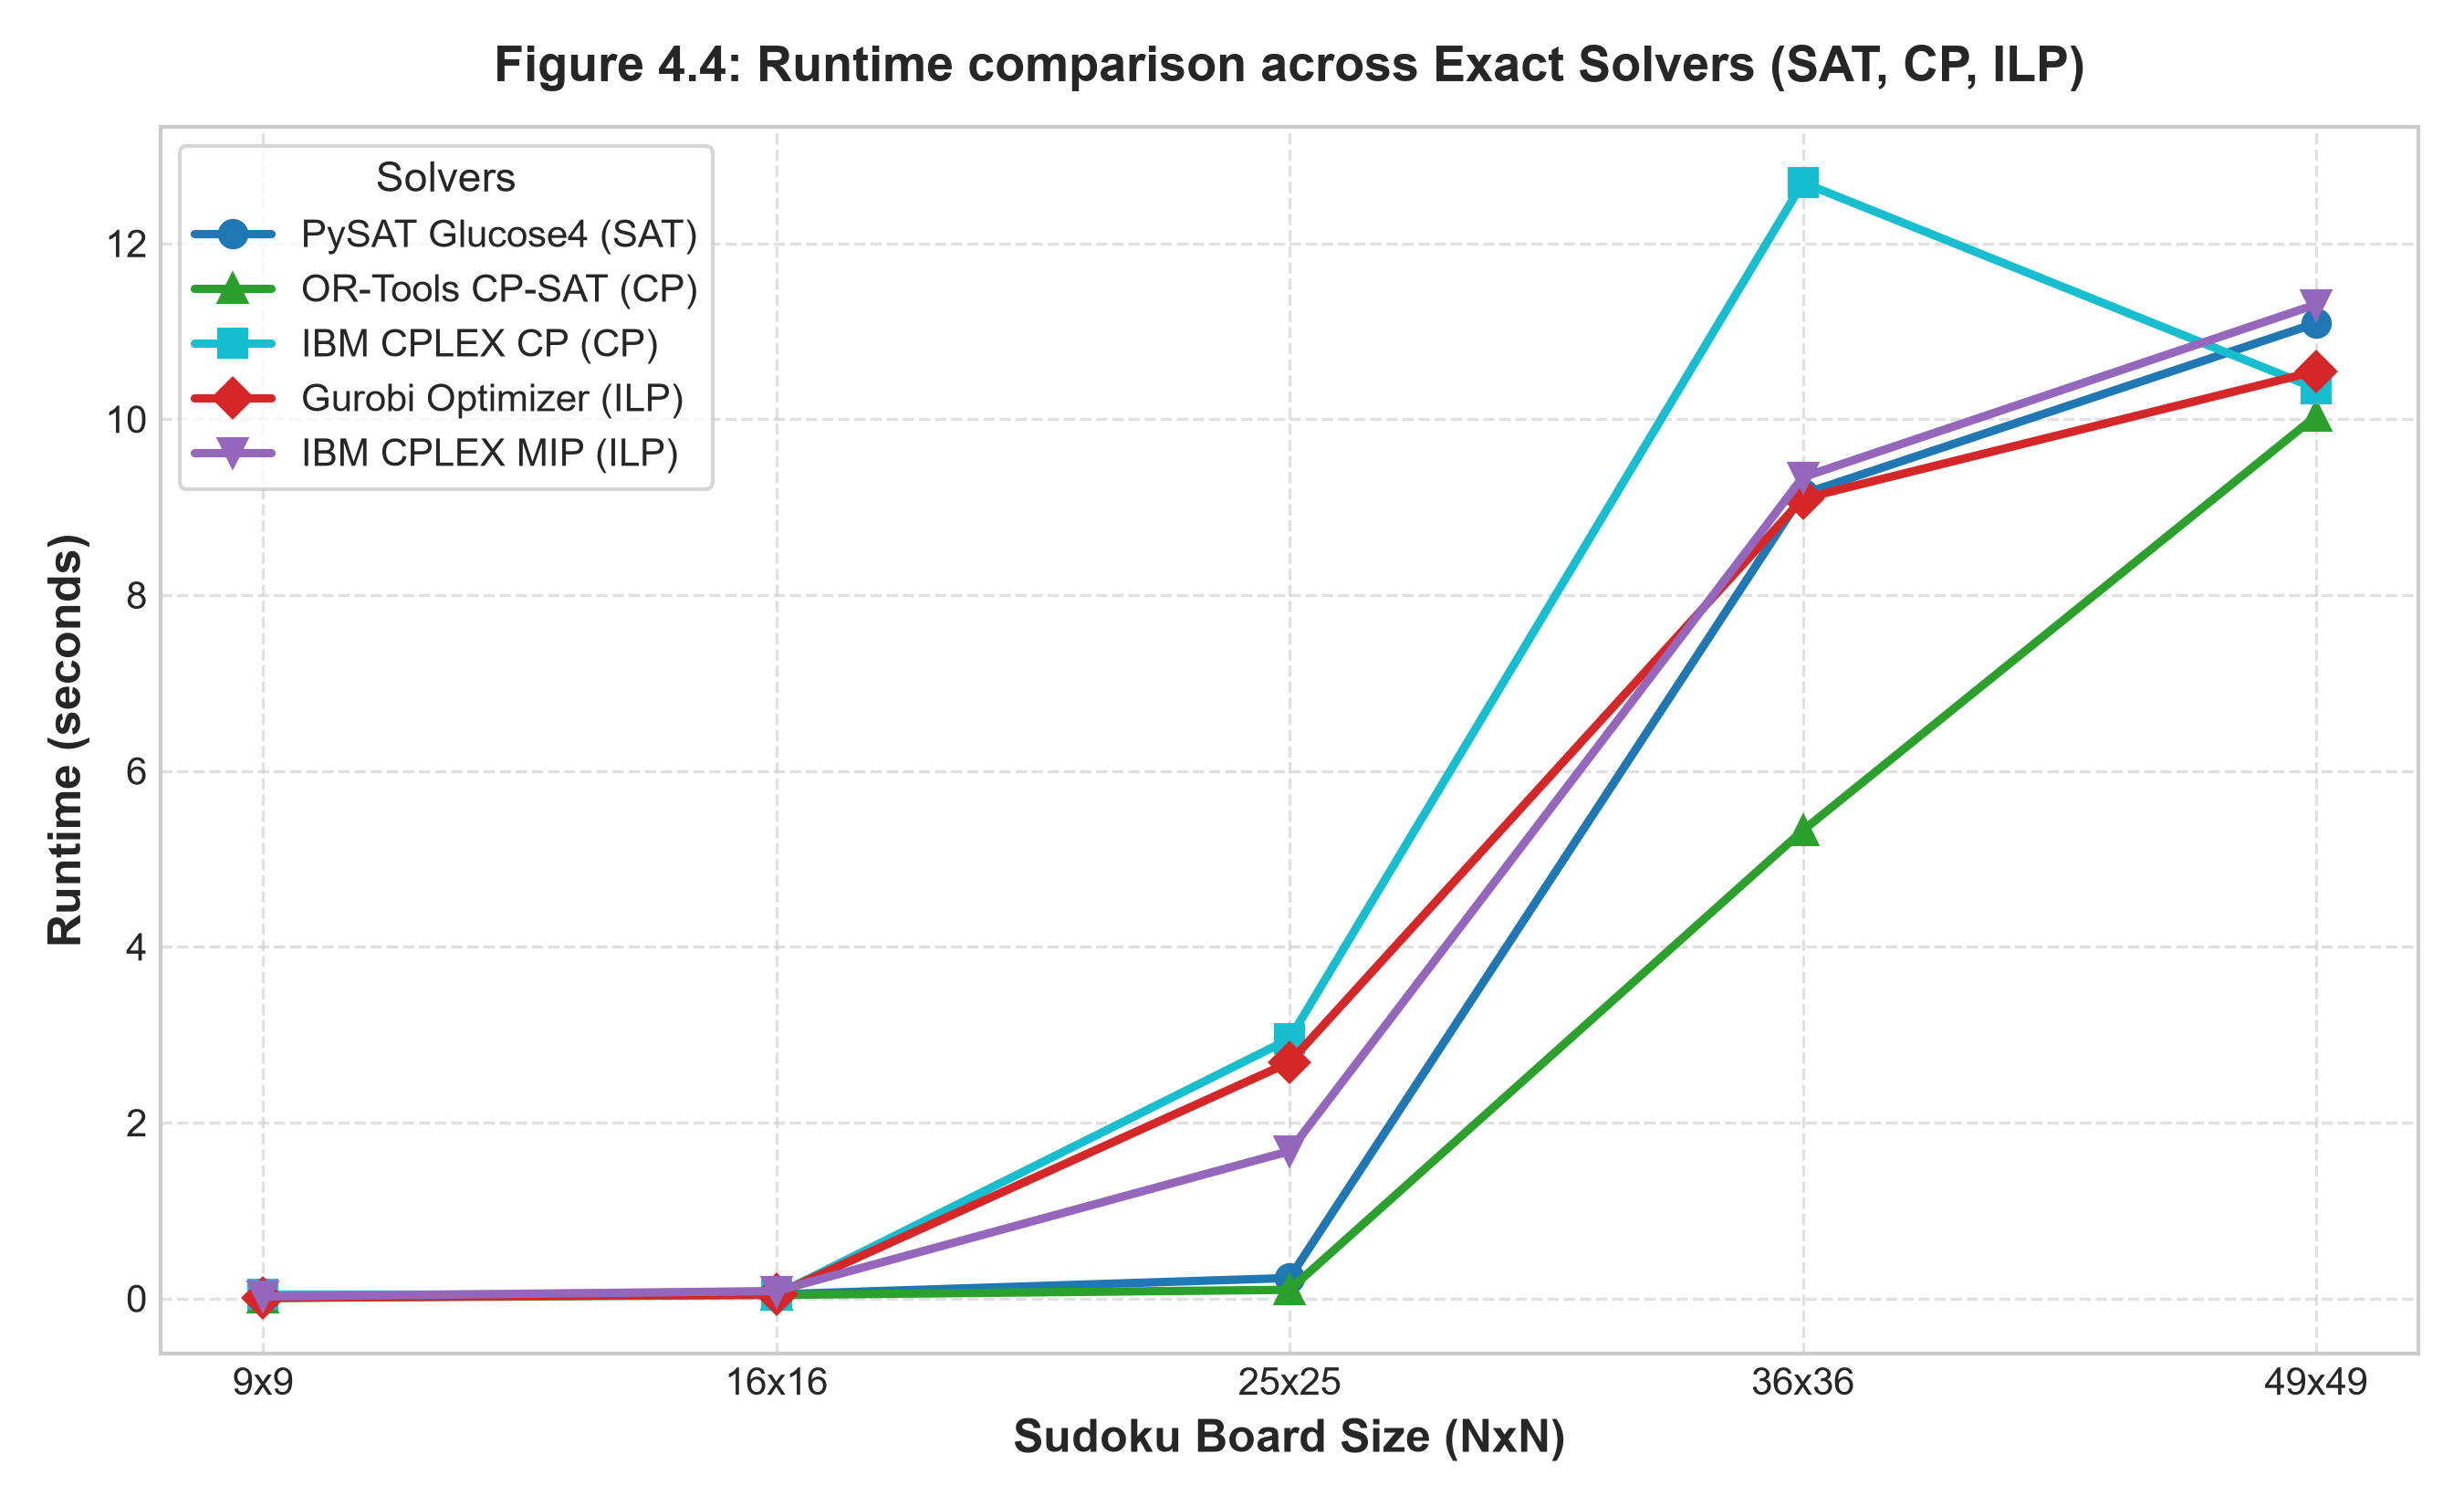
\includegraphics[width=0.58\textwidth]{fig_4_4_runtime_solvers.png}
    \vspace{2mm}
    \caption{Cross-paradigm runtime comparison across grid sizes under tiered timeouts (PAR-1 metric).}
    \label{fig:runtime_solvers}
\end{figure}

\subsection{Key Insights and Discussion}
Detailed comparative analysis of the experimental results yields six key insights:

\begin{enumerate}
    \item \textbf{Formula Size Complexity (Figures~\ref{fig:clauses_comparison} and~\ref{fig:variables_comparison})}: An $N \times N$ generalized Sudoku puzzle requires At-Most-One (AMO) constraints on $4N^2$ separate groups of $N$ variables: $N^2$ cell constraints, $N^2$ row constraints, $N^2$ column constraints, and $N^2$ block constraints.
    \begin{itemize}
        \item \textit{Clause Growth in Figure~\ref{fig:clauses_comparison}}: Under Binomial (Pairwise) encoding, each group produces $\binom{N}{2} = \frac{N(N-1)}{2}$ binary clauses without auxiliary variables. Across the whole board, this results in $4N^2 \times \frac{N(N-1)}{2} = 2N^3(N-1) = \mathcal{O}(N^4)$ total clauses. When $N = 49$, this fourth-power growth ($\mathcal{O}(N^4)$) causes the formula to explode to about $11.3$ million clauses ($2 \times 49^3 \times 48$), creating the steep curve in Figure~\ref{fig:clauses_comparison}. In contrast, linear encodings (Product and Sequential Counter) require only $\mathcal{O}(N)$ clauses per group, limiting the total clause growth to $4N^2 \times \mathcal{O}(N) = \mathcal{O}(N^3)$. This reduces the total number of clauses by a factor of roughly $N/2$ (from 11.3 million down to 1.35 million on $49 \times 49$).
        \item \textit{Total Variables in Figure~\ref{fig:variables_comparison}}: Figure~\ref{fig:variables_comparison} plots the \textbf{total variable count}, which is the sum of the $N^3$ base variables ($x_{r, c, v}$) and any auxiliary variables added by the encoding. Binomial encoding uses no auxiliary variables, staying strictly at $N^3$ base variables ($117,649$ at $N = 49$). In contrast, Sequential Counter adds $N - 1$ auxiliary variables per group (about $4N^3$ extra variables), bringing the total to $578,641$ variables at $49 \times 49$. Product encoding finds a practical middle ground: by arranging variables into a 2D grid, it introduces only $2\lceil\sqrt{N}\rceil$ auxiliary variables per group, resulting in a moderate total of $252,105$ variables.
    \end{itemize}

    \item \textbf{Why Lazy Clause Generation (LCG) Works Best}: Google OR-Tools CP-SAT was the best performer across all grid sizes in both speed and success rate. This result demonstrates the strength of Lazy Clause Generation (LCG)~\cite{feydy2009lazy}. Traditional CP solvers handle constraints like \texttt{AllDifferent} efficiently using domain filtering, but they cannot record the root causes of past conflicts. On the other hand, pure SAT solvers are very good at learning from conflicts using CDCL, but they require a huge number of clauses to encode constraints with many variables. OR-Tools CP-SAT combines the strengths of both approaches: it keeps a compact model with only $N^2$ integer variables and generates clauses dynamically only when a conflict occurs. This allows CP-SAT to avoid searching dead ends repeatedly, achieving a 90\% success rate on $36 \times 36$ grids where pure CP and ILP solvers struggle.
    
    \item \textbf{The Runtime Peak of CPLEX CP on $36 \times 36$ Grids}: In Figure~\ref{fig:runtime_solvers}, IBM CPLEX CP shows an unexpected pattern: its average runtime on $36 \times 36$ (12.69 s) is higher than on $49 \times 49$ (10.35 s). Looking closely at the experimental logs reveals three main reasons:
    \begin{itemize}
        \item \textit{Harder Puzzles in the $36 \times 36$ Dataset}: Half of the $36 \times 36$ puzzles had 45\% to 50\% blank cells, making them very hard to solve. In contrast, the $49 \times 49$ dataset had fewer blank cells (80\% of instances had 38\% or fewer blank cells). Therefore, the $36 \times 36$ test set contained relatively harder puzzles.
        \item \textit{Search Dead Ends in Classical CP}: CPLEX CP uses standard domain filtering without learning conflict clauses. When over 45\% of the cells are empty, simple logical deductions run out quickly. Because it cannot learn from conflicts and skip bad branches, CPLEX CP gets stuck repeatedly testing invalid values (known as thrashing).
        \item \textit{Penalty Time from Timeouts}: On $36 \times 36$ grids, CPLEX CP timed out on 7 out of 20 puzzles (a 35\% timeout rate). Under the 35 s limit, these timeouts alone added $7 \times 35\text{ s} / 20 = 12.25\text{ s}$ to the average runtime (total: 12.69 s). On $49 \times 49$ grids, CPLEX CP timed out on only 2 out of 10 puzzles (20\% timeout rate), adding $2 \times 50\text{ s} / 10 = 10.00\text{ s}$ of penalty time (total: 10.35 s). The higher failure rate on the harder $36 \times 36$ puzzles directly explains this runtime peak.
    \end{itemize}
    
    \item \textbf{High Efficiency of Linear-Clause SAT Encodings}: On $25 \times 25$ grids, pure SAT (Glucose4 with Sequential Counter) solved all instances in an average of 231.77 ms, running over 7 to 11 times faster than commercial ILP solvers (CPLEX MIP at 1,674 ms and Gurobi at 2,684 ms). This shows that once quadratic clause growth is avoided using linear encodings (such as Product or Sequential Counter), modern SAT solvers are extremely fast and effective for Sudoku-like problems.
    
    \item \textbf{Limitations of Linear Relaxations in ILP Solvers}: Commercial ILP solvers (Gurobi and CPLEX MIP) are very fast on small grids ($9 \times 9$ and $16 \times 16$) because their presolve step quickly fills in obvious cell values. However, on larger grids ($N \ge 25$), their performance drops significantly. Sudoku is a feasibility problem with no objective value to minimize or maximize. When an ILP solver relaxes the binary variables ($0$ or $1$) to continuous values between $0$ and $1$, it easily satisfies the equations by assigning fractional values (such as $1/k$) to many cells. These fractional solutions provide little useful guidance, forcing the solver to search blindly through thousands of binary variables ($117,649$ variables at $49 \times 49$) without effective pruning.
    
    \item \textbf{Memory Usage and CPU Cache Limits}: The slow performance of Binomial SAT on large grids is also related to computer hardware. At $49 \times 49$, the 11.3 million clauses generated by Binomial encoding require more than 200 MB of memory. Because this is much larger than the CPU cache (the test machine has a 12 MB L3 cache), the processor must repeatedly fetch clauses from slower system RAM. In contrast, linear encodings (Product and Sequential Counter) generate only about 1.35 million clauses ($\approx 20\text{ MB}$), fitting much better in fast cache memory and allowing the SAT solver to check clauses much faster.
\end{enumerate}

\clearpage
% =========================================================================
% 5. CONCLUSION
% =========================================================================
\section{Conclusion}
\label{sec:conclusion}

This paper presented an experimental comparison of exact solving methods for generalized Sudoku puzzles up to $N = 49$. Across 46,530 test runs, we evaluated five SAT At-Most-One (AMO) encodings alongside commercial ILP solvers (Gurobi, CPLEX MIP), CPLEX CP, and Google OR-Tools CP-SAT.

Our findings show that while the simple Binomial encoding works well for standard $9 \times 9$ boards, larger grids require linear-clause encodings like Product or Sequential Counter to prevent the clause count from growing out of control. Furthermore, across all tested solvers, Google OR-Tools CP-SAT delivered the best overall speed and reliability, showing that Lazy Clause Generation is an effective approach for this type of constraint problem. Future work could investigate symmetry breaking and additional preprocessing techniques for even larger boards.

\section*{Data Availability}
The benchmark dataset, scripts, and complete experimental result logs used in this study are openly available in the project repository: \url{https://github.com/xXor4nd/Sudoku_Project/}.

\clearpage
% =========================================================================
% REFERENCES
% =========================================================================
\begin{thebibliography}{8}

\bibitem{SAT_book}
T.~V.~Khanh, K.~V.~Tuyen, T.~X.~Hieu, V.~T.~Huong, D.~X.~Nghia, and N.~T.~K.~Duc.
\newblock {\em Chuyen khao: Bieu dien SAT toi uu cho cac bai toan toi uu hoa to hop -- Phan 1: Nen tang va tieu chi thiet ke} [Monograph: Optimal SAT Representations for Combinatorial Optimization Problems -- Part 1: Foundations and Design Criteria].
\newblock Monograph, July 2026.

\bibitem{khanh_lecture_slides}
T.~V.~Khanh.
\newblock {\em Lecture Slides: Module 1 (Propositional Logic), Module 2 (SAT Encodings), and Module 3 (AMO and ALO Encodings)}.
\newblock Course Lecture Notes, VNU University of Engineering and Technology, 2026.

\bibitem{royle2014minimum}
G.~Royle.
\newblock Minimum Sudoku: 17-clue puzzles.
\newblock University of Western Australia, 2014.

\bibitem{feydy2009lazy}
T.~Feydy and P.~J.~Stuckey.
\newblock Lazy clause generation re-engineered.
\newblock In {\em Principles and Practice of Constraint Programming -- CP 2009}, pages 352--366. Springer, 2009.

\bibitem{ignatiev2018pysat}
A.~Ignatiev, A.~Morgado, and J.~Marques-Silva.
\newblock {PySAT}: A {Python} toolkit for prototyping with {SAT} oracles.
\newblock In {\em Theory and Applications of Satisfiability Testing -- SAT 2018}, pages 428--437. Springer, 2018.

\bibitem{ortools}
L.~Perron and V.~Furnon.
\newblock {OR-Tools}: Google's software suite for combinatorial optimization.
\newblock \url{https://developers.google.com/optimization}, 2024.

\bibitem{gurobi2024}
Gurobi Optimization, LLC.
\newblock {\em Gurobi Optimizer Reference Manual}, 2024.
\newblock Version 11.0.

\bibitem{cplex2022}
IBM Corporation.
\newblock {\em IBM ILOG CPLEX Optimization Studio Reference Manual}, 2022.
\newblock Version 22.1.1.

\end{thebibliography}

\end{document}
